\section{APX-completeness for segments parallel to axis}
\label{section:segment_apx}

\subsection{Definition of  MAX-(3,3)-SAT problem}
Here we define MAXSAT problem.

\begin{tw}{
	\label{hastadtheorem}
	\textbf{\cite{hastad}}
	Assume NP $\not\subseteq$ $DTIME(2^{O(\log n \log \log n)})$.
	Then, there exists a constant $c > 0$, such that for
	$$\epsilon'(n) = \frac{c \log \log \log n}{\log \log n}$$ 
	fully satifiable 3-SAT formulas cannot be distinguished 
	in polynomial time from
	3-SAT formulas where no more than $(7/8+\epsilon'(n))n$ clauses
	can be satisfied in polynomial time.
}\end{tw}

\begin{lemma}{
	\label{apxconstruction}
	Given an instance of  MAX-(3,3)-SAT 
	with $n$ variables and optimal result $k$,
	we can construct an instance of axis-parallel segments in 2D,
	which optimal result (even with 1/2-extension) is exactly $15n - k$.
}\end{lemma}

\begin{tw}{
	\textbf{(axis-parallel segment set cover with 1/2-extension is APX-hard)}.	
	For sufficiently small $\epsilon > 0$,
	there does not exist an $(1+\epsilon)$-approximation scheme
	for unweighted geometric set cover
	with axis-parallel segments in 2D (even with 1/2-extension)
	(problem is APX-hard).
}\end{tw}

\paragraph{Proof.}
Take any $0 < \epsilon < 1/(15 \cdot 8)$.
Choose $n$ sufficiently large, so that $\epsilon'(n)$ from
Theorem \ref{hastadtheorem}
is not greater than $\epsilon$.

Let's assume that there exists an $(1+\epsilon)$-approximation scheme
for unweighted geometric set cover with axis-pararell segments in 2D.
We will construct an algorithm distinguishing instances of
MAX-(3,3)-SAT
in Theorem \ref{hastadtheorem}.
Take two instances to be distinguished and using
Lemma \ref{apxconstruction}
and name them satisfiable -- $S_1$ and unsatisfiable -- $S_2$.
Let's construct two instances of geometric set cover
and name them respectively $I_1$ and $I_2$.

Use $(1+\epsilon)$-approximation scheme for instances of geometric
set cover, let's name the result of this approximation
for an instance of problem $I$ as $approx(I)$.

From defintion of $S_1$ and $S_2$ we have:
$$OPT(S_1) = n$$
$$OPT(S_2) \le (\frac{7}{8} + \epsilon'(n))n$$

From Lemmma \ref{apxconstruction} we have:

$$OPT(I_1) = 14n$$
$$OPT(I_2) = 15n - (\frac{7}{8} + \epsilon'(n))n$$

Let's prove that $approx(I_2) > approx(I_1)$:

$$approx(I_2) \ge OPT(I_2) = 15n - (\frac{7}{8} + \epsilon'(n))n
	= 14n + (\frac{1}{8} - \epsilon'(n))n
	> 14n + (\frac{1}{8} - \epsilon)n > $$
$$	> 14n + (15\epsilon - \epsilon)n
	= 14n + (14\epsilon)n
	= 14n(1+\epsilon)
	= OPT(I_1)(1+\epsilon) \ge approx(I_1)$$ 



Therefore, by using out supposed $(1+\epsilon)$ approximation,
it’s possible to distinguish $S_1$ from $S_2$, since
the approximation scheme will always return a smaller value
for $I_1$ than for $I_2$. This is a contradiction,
hence the approximation scheme cannot exist.

\subsection{Reduction construction}
\label{reduction_construction}

Let's take some instance of  MAX-(3,3)-SAT with
variables $x_1, x_2 \ldots x_n$
and clauses $C_1, C_2 \dots C_n$.

We will create gadgets for choosing the value
of variables (\textit{true} or \textit{false}) and checking
if the clauses are met (any of the variables were chosen).

\begin{figure}[h]
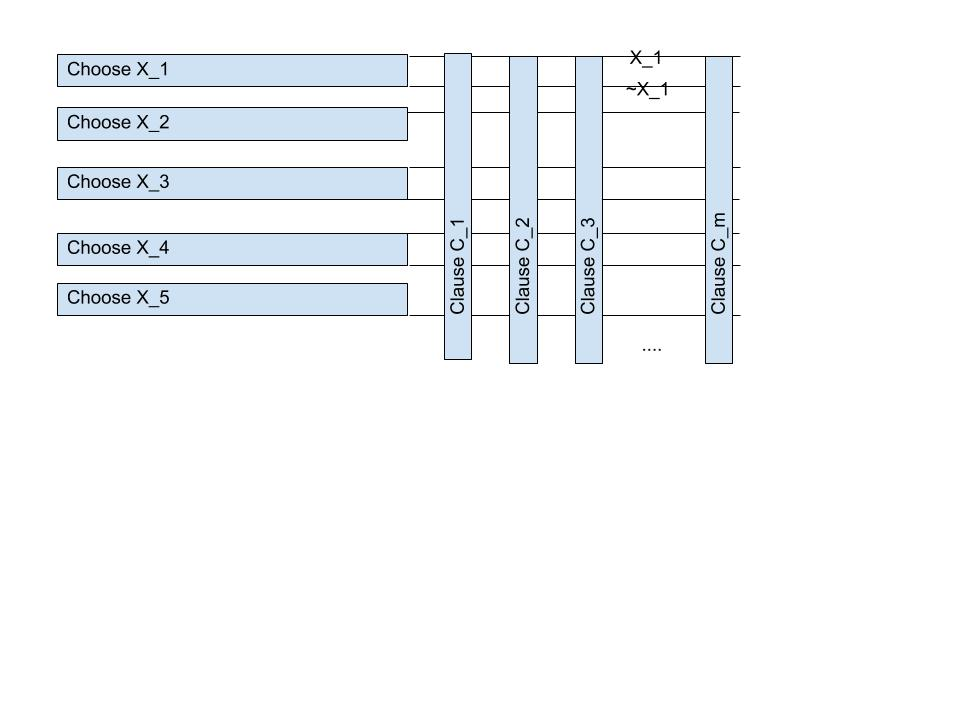
\includegraphics[width=0.7\textwidth]{segment_apx_sketch.jpg}
\caption{General scheme of reduction.}
\label{fig:segment_apx}
\end{figure}

\subsubsection{Choose $x_i$ gadget}
\begin{figure}[h]
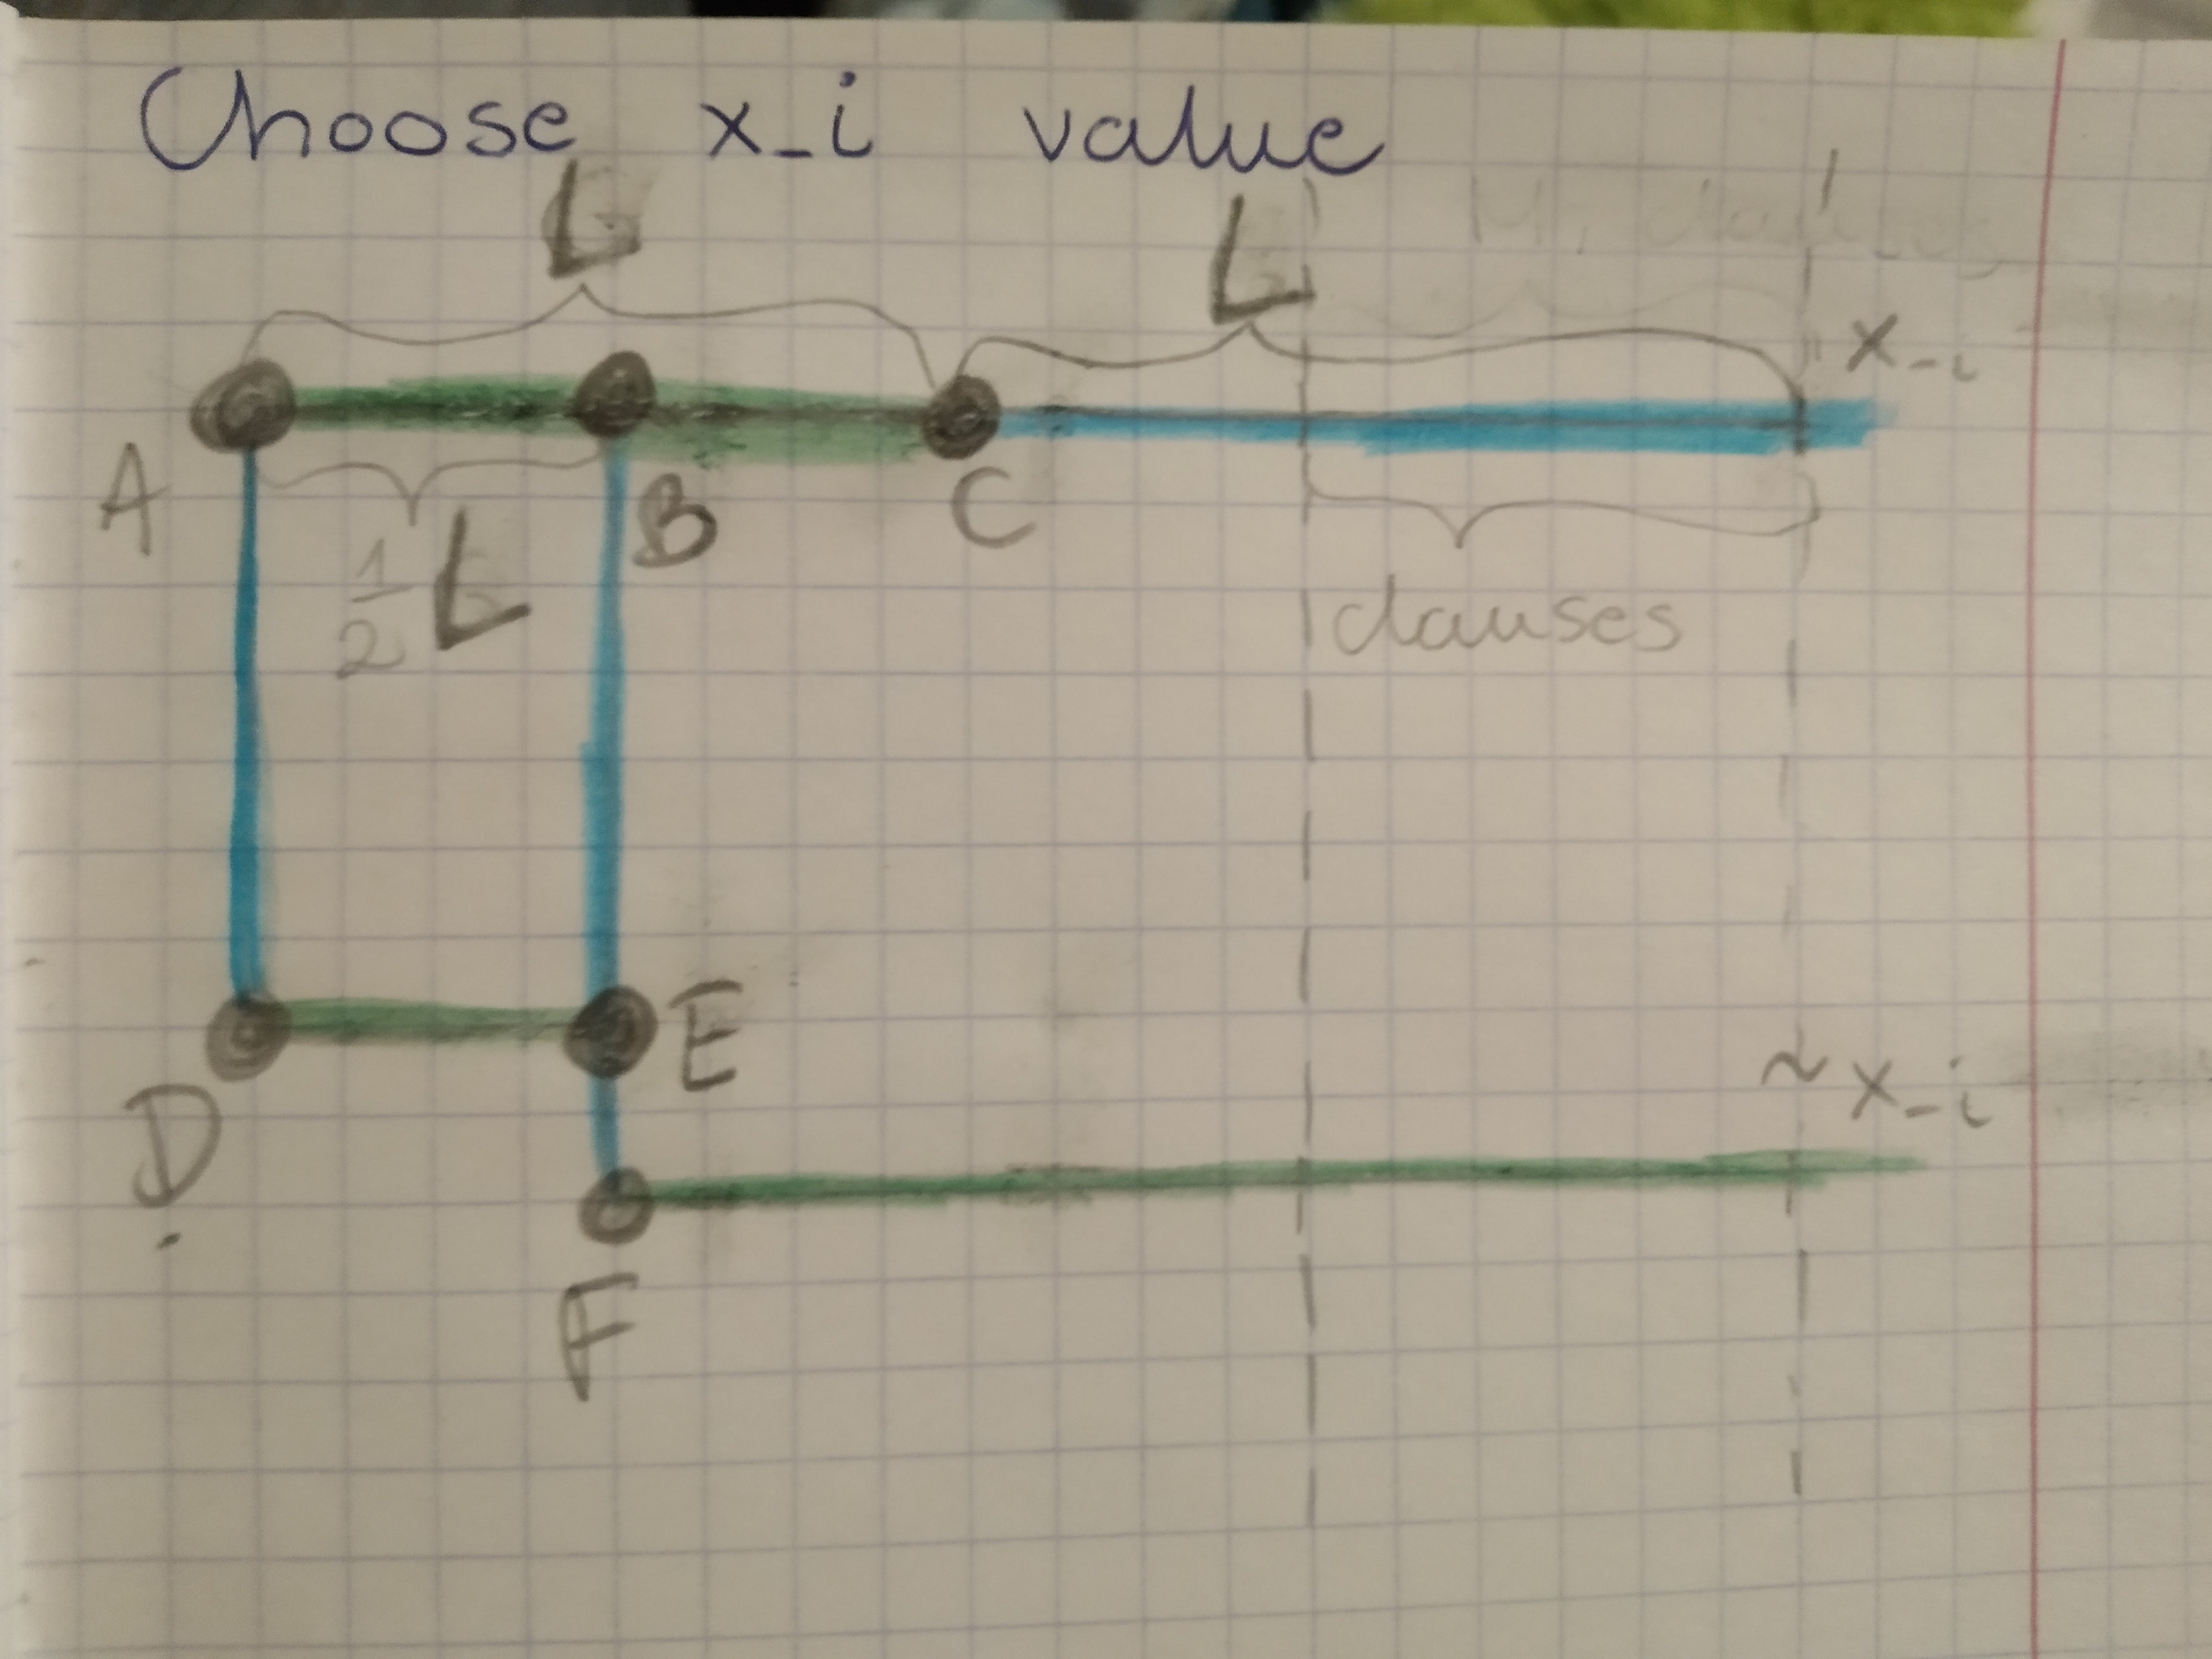
\includegraphics[width=0.6\textwidth]{choose_x_gadget.jpg}
\caption{Scheme of choose $x_i$ gadget.}
\label{fig:choose_x_gadget}
\end{figure}
In Figure~\ref{fig:choose_x_gadget},
we show a gadget that simulates a single variable $x_i$.
It consists of six points A, B, C, D, E, F, and several segments.
Selecting the segment marked with $x_i$
to the solution will correspond to setting $x_i$ to \textit{true},
while selecting the segment marked with $\neg x_i$
to setting $x_i$ to \textit{false}.
In the following lemmas,
we show that this construction indeed models a binary variable.

First, note that in the gadget
there are exactly two sets of three segments
that cover all points $A, B, C, D, E, F$.
These two sets of segments are marked in
Figure~\ref{fig:choose_x_gadget} in blue and green, respectively.

\begin{lemma}
\label{choose_variables_no_less}
Points $A, B, C, D, E, F$ cannot be covered using less than
3 segments (even with $1/2$-extensions).
\end{lemma}
\paragraph{Proof.}
We need to take at least one segment on line $ABC$,
because it's the only way to cover $C$.
All other points ($D, E, F$) are not colinear,
so we need at least 2 other segments to cover them.

\begin{lemma}
\label{choose_variables_both}
If we choose both segments $x_i$ and $\neg x_i$, we need to use at
least 4 segments to cover all points $A, B, C, D, E, F$
(even with $1/2$-extensions).
\end{lemma}


\paragraph{Proof.}
Choosing both segments $x_i$ and $\neg x_i$
we only cover points $C$
(becuase $B$ is too far away to be covered with $1/2$-extension)
and $F$.

The remaining points ($A, B, D, E$) are not colinear,
so we need at least two more segments to cover them.


\begin{lemma}
\label{choose_variables_solution}
There exist a solution such that takes a segment $x_i$ ($\neg x_i$)
and 2 other segments, and covers all points $A, B, C, D, E, F$
\end{lemma}

\paragraph{Proof.}
We can choose $x_i$, $AD$ and $BF$.

Alternatively we can choose $\neg x_i$, $AC$, $DE$.

\paragraph{Robustness to $1/2$-extension.}
Take a look at Figure~\ref{fig:segment_apx}.
The points will be included in choose gadgets (horizontal boxes)
and clause gadgets (vertical boxes).

Since segment $AC$ is very long
and colinear with $x_i$, after $1/2$-extension
it will cover a significant part of segment $x_i$,
even though $x_i$ will not be chosen.

If we put all the clause gadgets in the area
marked with \textbf{clauses} at gadget scheme in Figure~\ref{fig:choose_x_gadget},
it is enough to prove that $AC$ will not cover any points
in the \textbf{clauses} area even with $1/2$-extensions.

\begin{lemma}
No points in \textbf{clauses} area can be covered
by $AC$ with $1/2$-extension.
\end{lemma}

\paragraph{Proof.}
Bear in mind that length of $AC$ is equal to length of $x_i$.
Area \textbf{clauses} takes a second half
of the segment $x_i$ and $AC$ after extension will cover the first
half of segment $x_i$.

\subsubsection{Clause gadget}
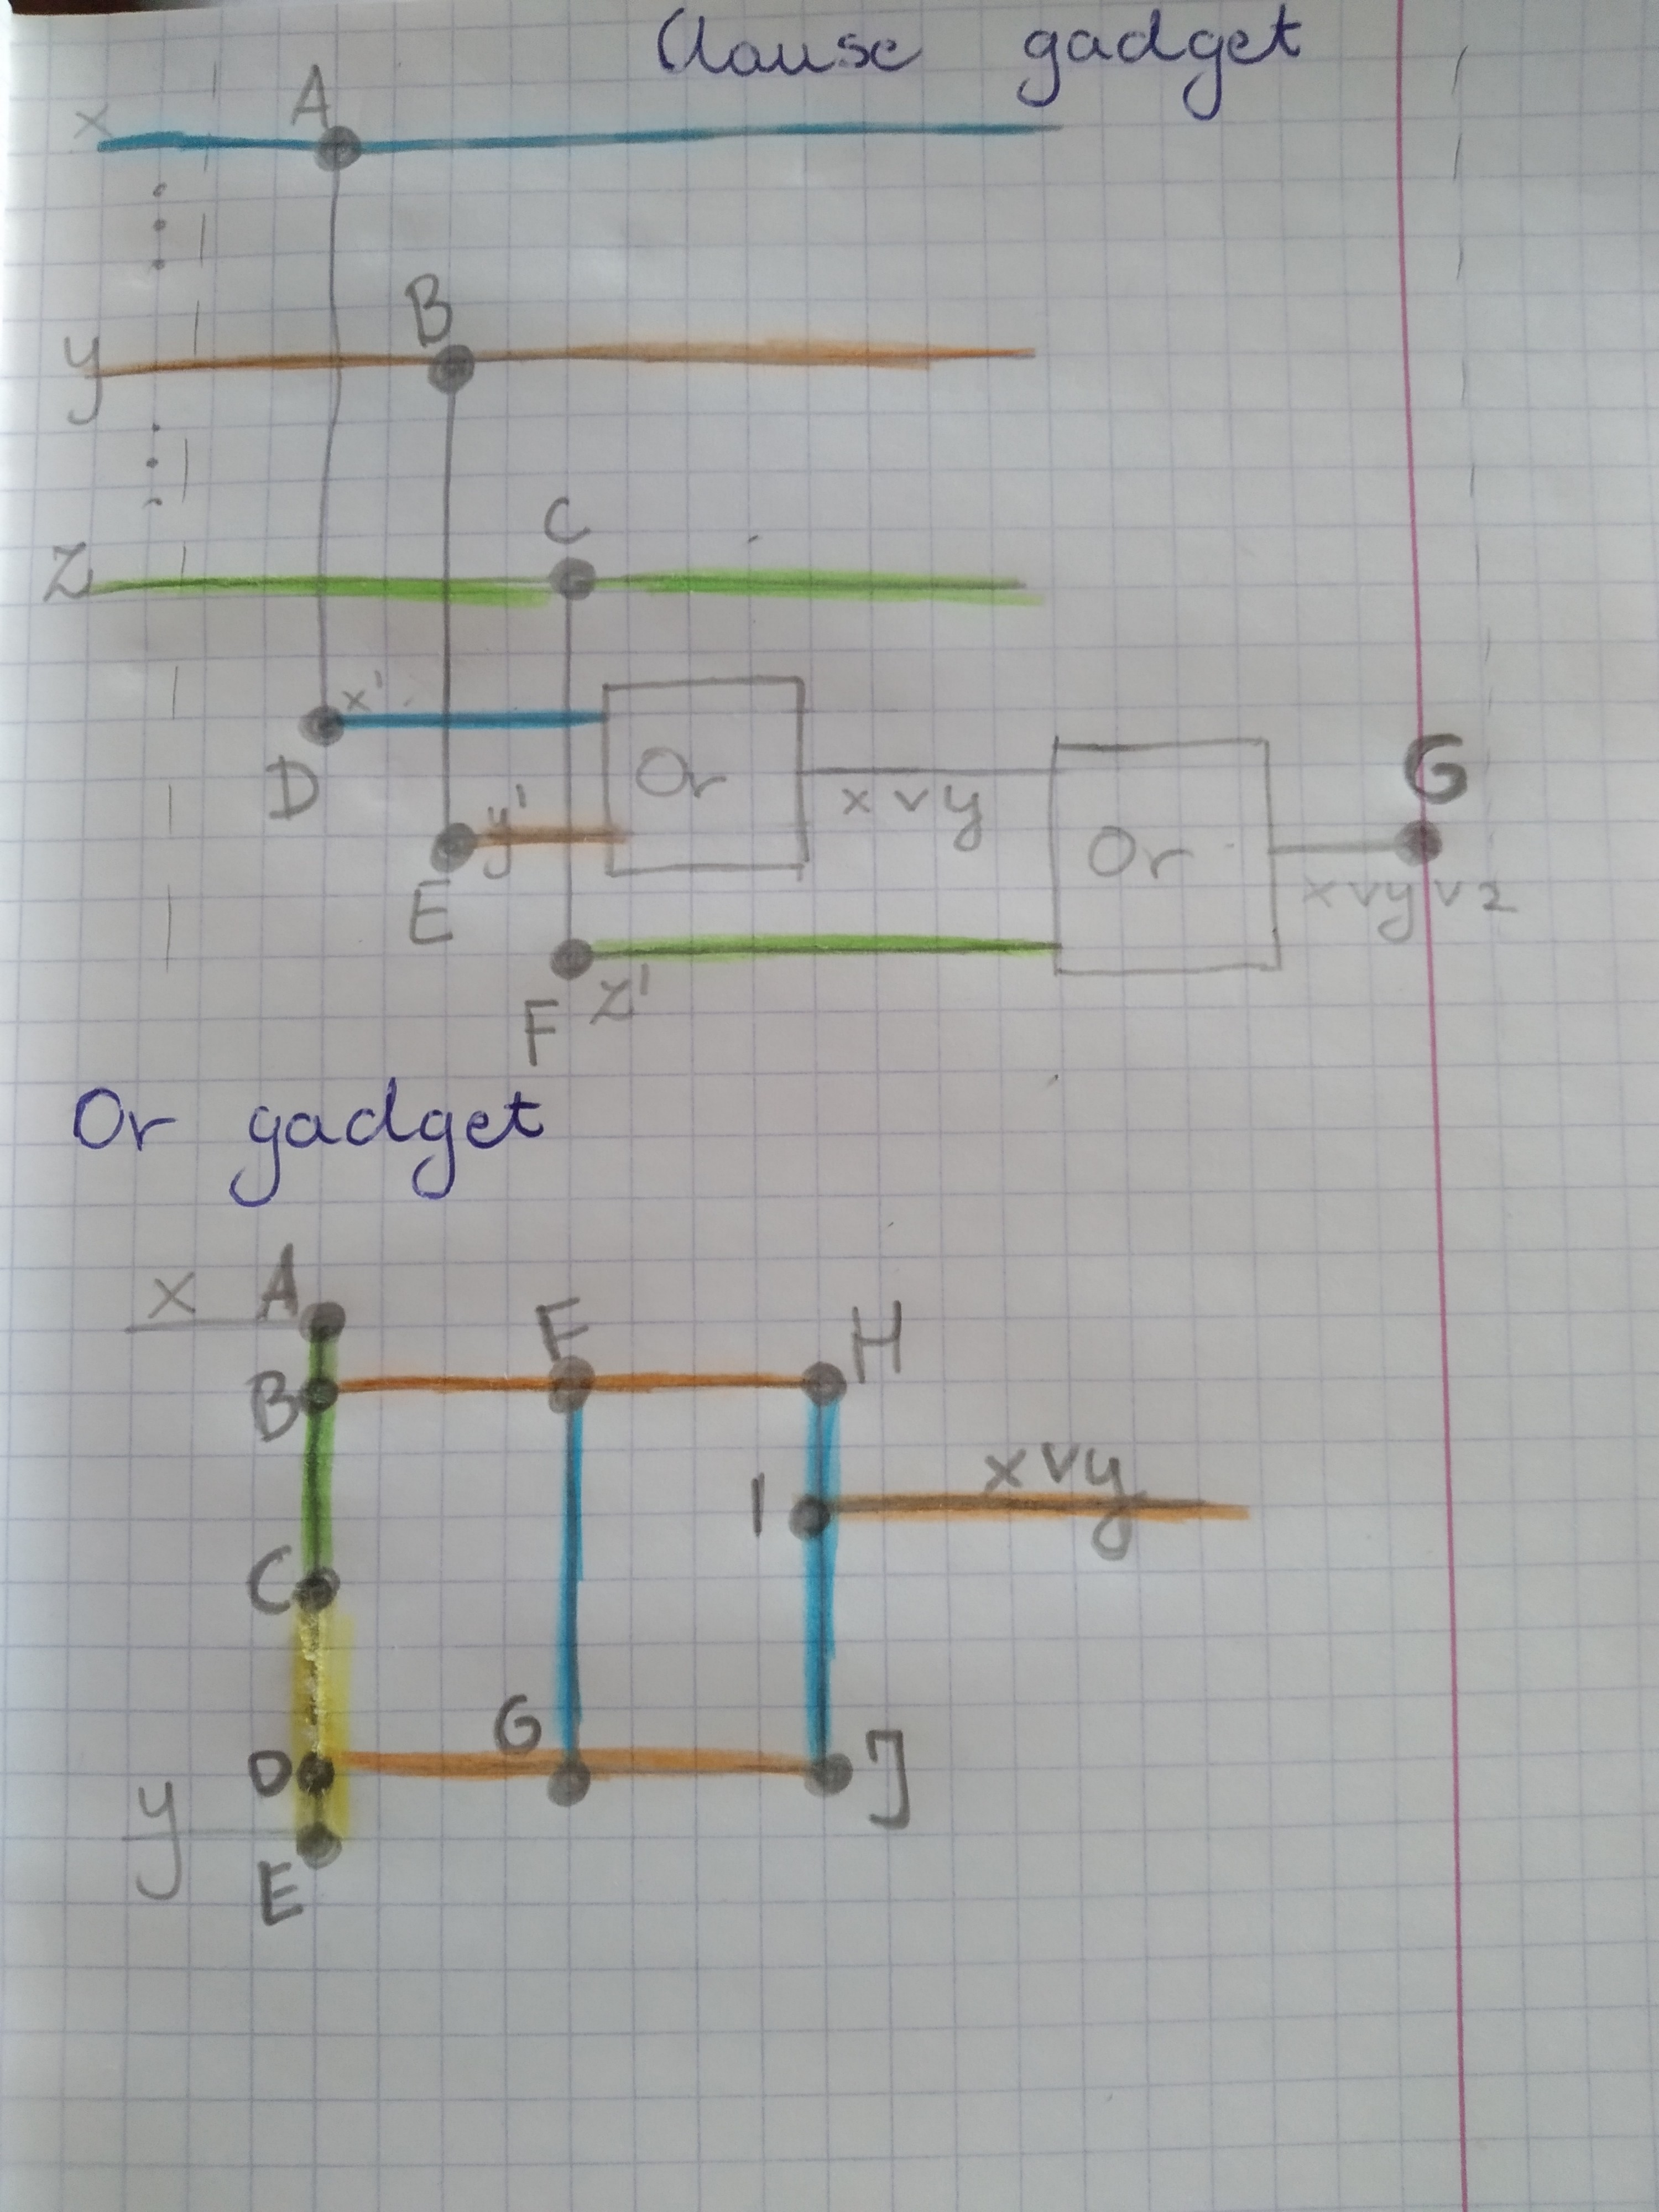
\includegraphics[width=0.6\textwidth]{clause_gadget.jpg}

\begin{lemma}
In order to cover $D$ ($E, F$) point at least one
of the segments $AD$ ($BE, CF$) or $x'$ ($y', z'$).
\end{lemma}

\begin{lemma}
Points $A$ and $D$ can be covered
with one additional segment $x'$
only if $x$ is already chosen.
Otherwise they can be covered with one segment
only by using $AD$.
\end{lemma}

\begin{lemma}
\label{cover_or_gadget_no_less}
Points $A, B, C, D, E, F$ can be covered with 
3 segments and cannot be covered in less even with $1/2$-extension.
\end{lemma}

\paragraph{Proof.}
There are 3 points that aren't pairwise connected,
so they have to be covered with 3 separate segments.

Also there exists solution with 3 segments, ie. $AD$, $BE$, $CF$.

\subsubsection{Or gadget}
\begin{lemma}
\label{cover_clauses_segments_no_less}
Points $A, B, C, D, E, F, G, H, I, J$ can be covered using
at least 4 segments and cannot be covered with less
even with $1/2$-extension.
\end{lemma}

\begin{lemma}
Points $A, B, C, D, E, F, G, H, I, J$ can be covered using
4 segments and segment $x \lor y$ can be chosen
even with $1/2$-extension
only if at least one of the segments $x$ or $y$ is chosen.
\end{lemma}

\begin{lemma}
\label{cover_clauses_segments_no_less}
The whole caluse gadget can be covered with 11 segments and
cannot be covered with less
even with $1/2$-extension.
\end{lemma}

\begin{lemma}
\label{cover_clauses_solution}
The whole caluse gadget can be covered with 11 segments and
only when one of the variables $x, y$ or $z$ is chosen,
otherwise it can be covered with 12 segments.
\end{lemma}

\subsection{Proofs of construction Lemma \ref{apxconstruction}}
\begin{lemma}
	\label{construction_correctness}
	Given an instance of MAX-(3,3)-SAT of size $n$
	with optimal solution $k$.
	For instance of geometric cover, constructed
	in the aforementioned manner, 
	there exists a solution of weight $15n - k$.
\end{lemma}
\paragraph{Proof.}
Let's name the assignments of the variables in MAX-(3,3)-SAT instance,
that achieve the optimal solution,
$y_1$,~$y_2$~$\ldots$~$y_n$,
Let's cover every clause with solution described in
Lemma~\ref{choose_variables_solution},
in the $i$-th segment choosing the segment responsible for value $y_i$.

Cover every clause gadget with solution described in
Lemma~\ref{cover_clauses_solution}.

This solution uses $3n + (11m + (m-k)) = 15n - k$ segments.

\begin{lemma}
	\label{construction_completness}
	Given an instance of MAX-(3,3)-SAT of size $n$,
	and solution of size $w$ to the instance of geometric cover,
	constructed in the aforementioned manner, 
	there exists a solution to MAX-(3,3)-SAT of size at least $15n - w$.
\end{lemma}
\paragraph{Proof.}
Among the segments responsible for choosing the value of variable $x_i$,
we need to use at least 3 segments (Lemma~\ref{choose_variables_no_less}).
If we have chosen segments responsible for both $x_i$ and $\neg x_i$,
then we have used at least 4 segments (Lemma~\ref{choose_variables_both}).

If we chose at most one of the variables $x_i$ and $\neg x_i$,
choose that value to the solution. If we chose both values,
choose the value that appears in most (at least 2) clauses.
If we have chosen none of the values, choose any value.

To cover these segments we have used at least $3n + a$ segments,
where $a$ is the number of variables that we have chosen both
values for.

Among the segments responsible for the clause $C_i = x \lor y \lor z$
we need to use at least 11 segments
(Lemma~\ref{cover_clauses_segments_no_less})
and if we can cover it with 11 segments, then we have 
earlier chosen
one of the variables $x$, $y$ or $z$.

So we have 11 segments for satisfied clauses and 12 segments
for unsatisfied clauses, so we cover it with 
at least $11n + b$ segments, where $b$ is number of clauses
where none of the variables $x, y, z$ were chosen.
If the segment responsible for $x$ was taken,
but this variable is set to have this value,
then we have chosen both $x$ and $\neg x$ for this variable,
so "we cheated" and this maybe clause is not met,
but we assigned the value for this $x_i$ that meets
the most clauses, so for each of this variables,
at most one of the clauses isn't met.

So there are at most $a+b$ unsatsfied clauses in this instance,
so we have shown the resultwith result at least $n-(a+b)$.

$$w > 3n + a + 11n + b = 14n + a + b$$
$$15n - w < n - (a+b)$$

\subsubsection{Proof of Lemma \ref{apxconstruction}}
Given an instance of MAX-(3,3)-SAT of size $n$
with optimal result $k$.
Let's construct an instance of geometric cover,
constructed in aforementioned manner.

Given the Lemma~\ref{construction_correctness}, we know
the optimal solution for the constructed geometric cover is
at most $17n - k$ and since the $k$ is optiomal solution
for MAX-(3,3)-SAT, then according to Lemma~\ref{construction_completness}
there doesn't exist a solution with cost lesser than $17n - k$.
